\chapter{PCA Data Driven Surrogate Signal Extraction Methods for Dynamic PET Results With and Without Pre- and Post-Processing} \label{sec:pca_data_driven_surrogate_signal_extraction_methods_for_dynamic_pet_results_with_and_without_pre_and_post_processing_appendix}
    \newpage

    \begin{figure}
        \centering
        
        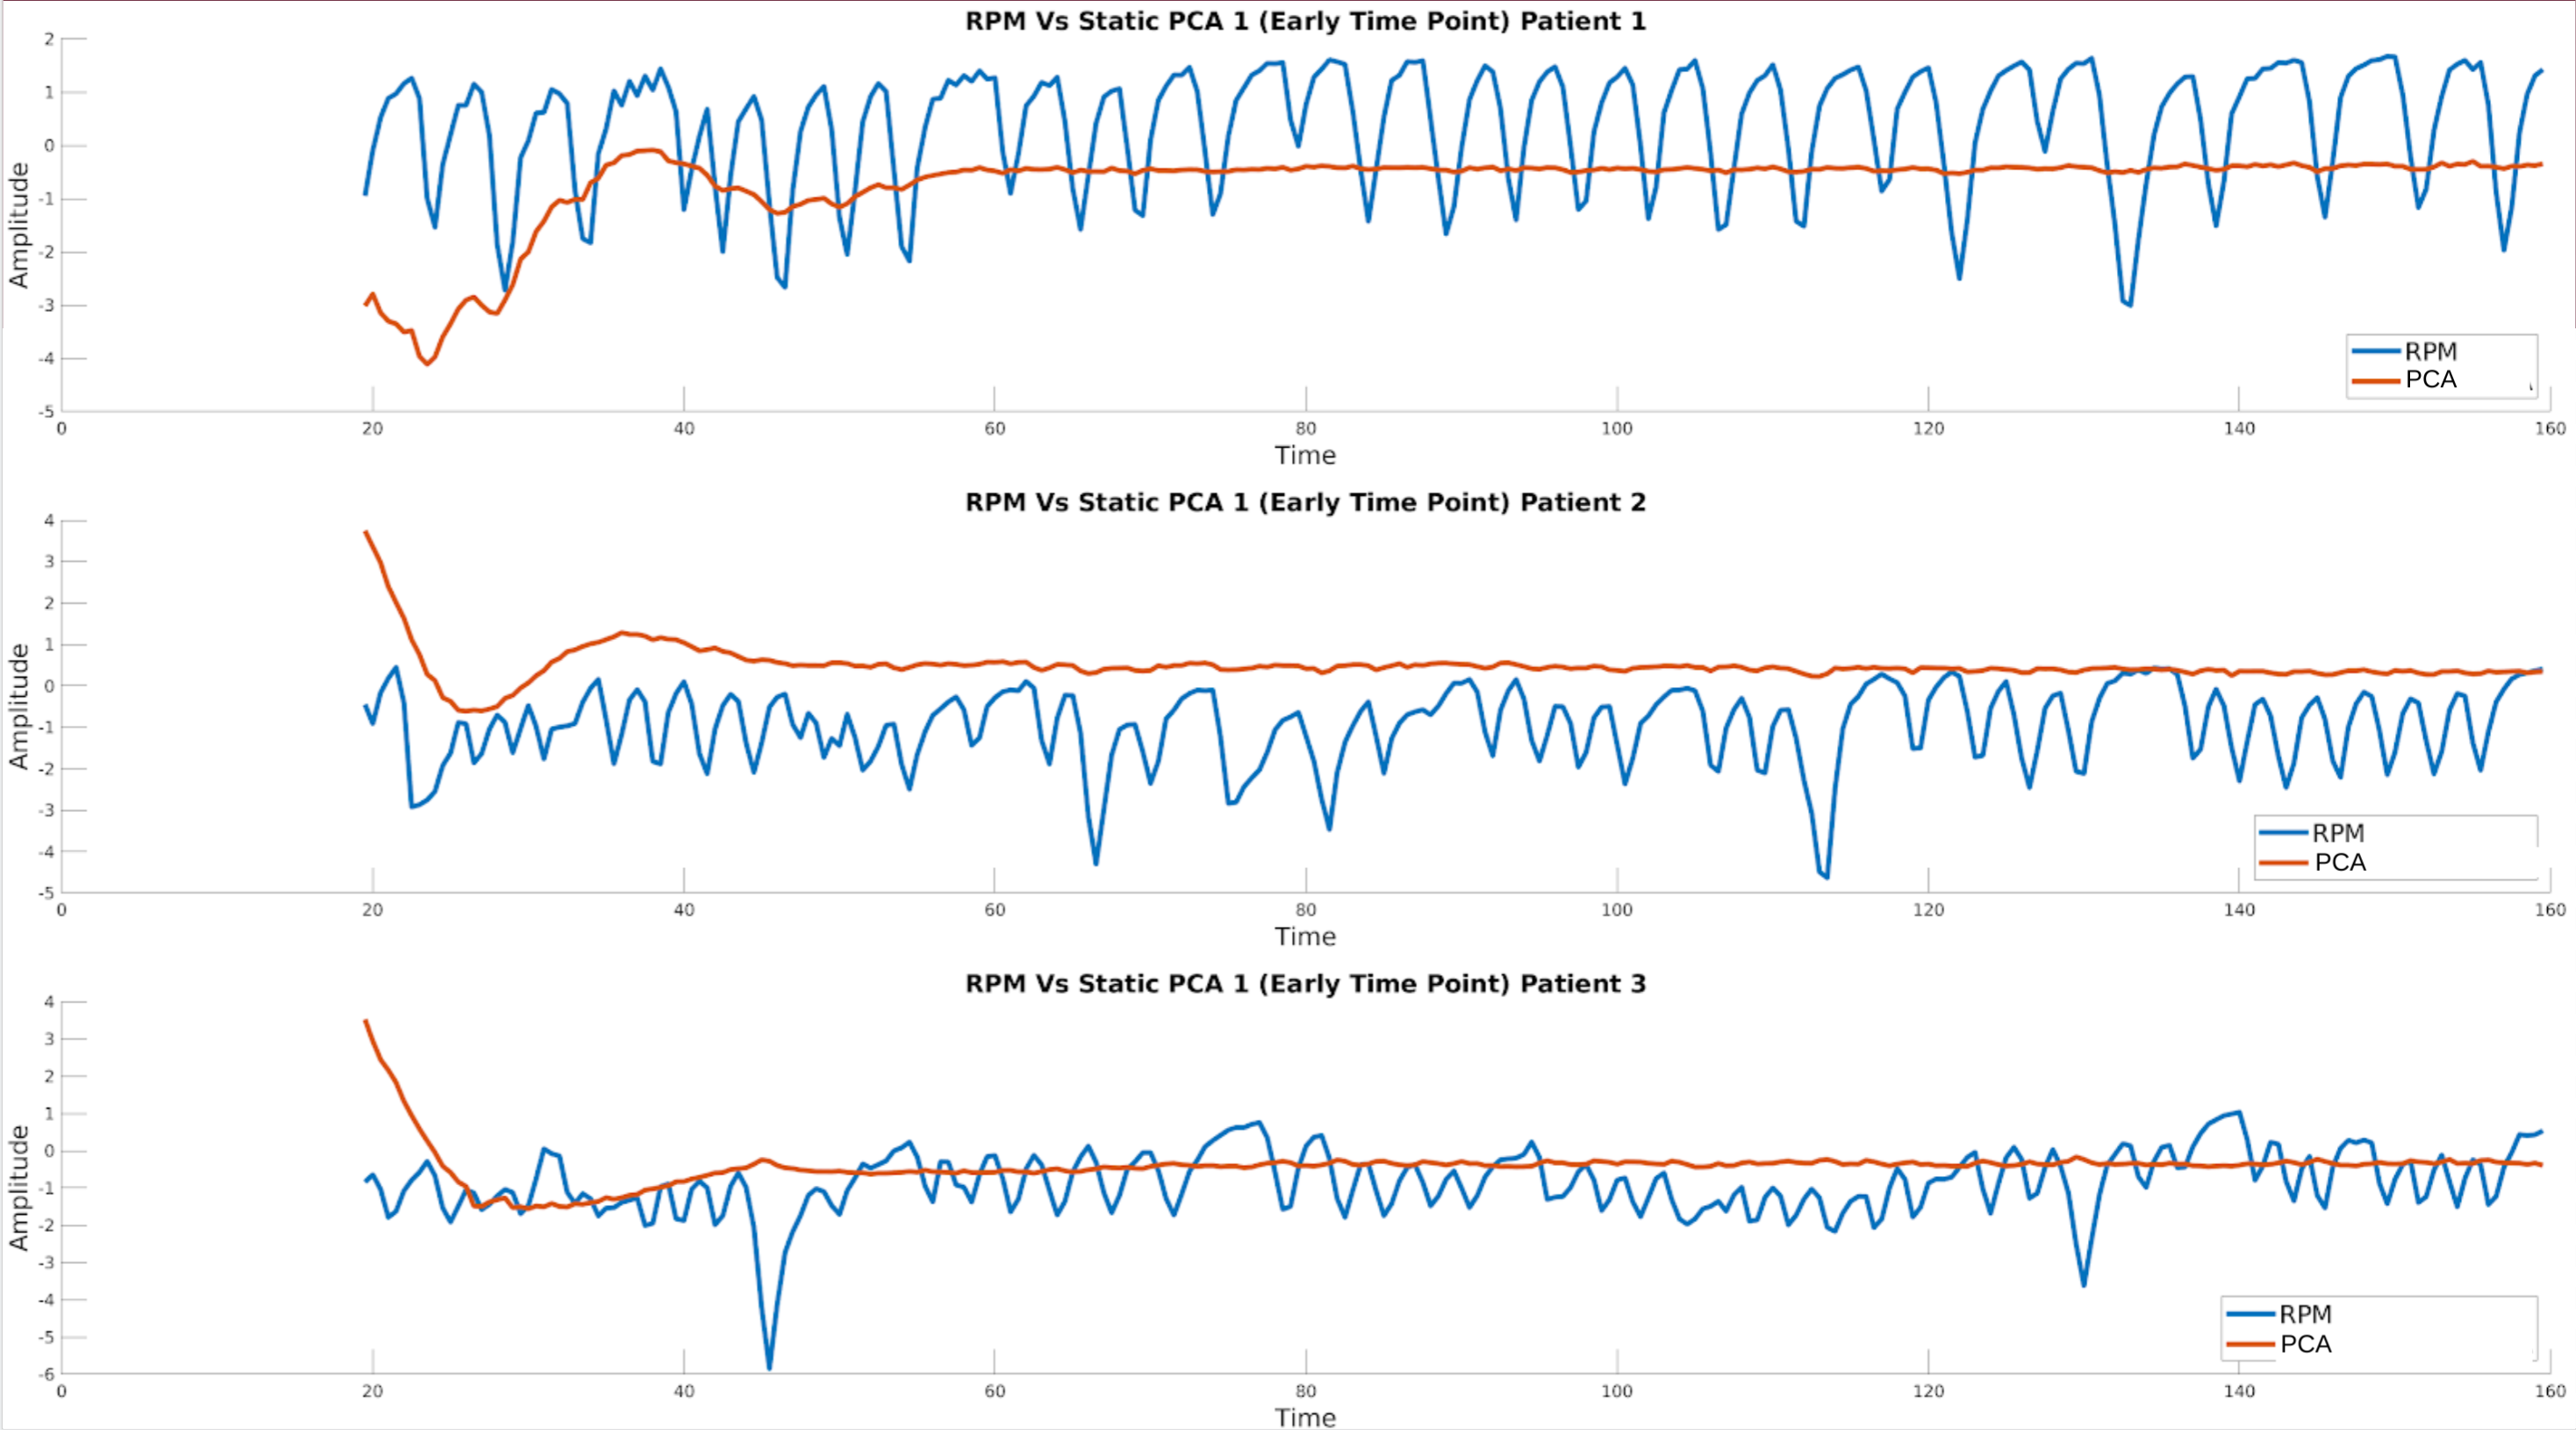
\includegraphics[width=1.0\linewidth]{figures/data_driven_surrogate_signal_extraction_results_1_vanilla_surrogate_signal.png}
        
        \captionsetup{singlelinecheck=false}
        \caption{
            A visual comparison between the \gls{RPM} \gls{SS} and the \gls{SS} from the static \gls{PCA} method using only the first \gls{PC} for three patients between \SI{20}{\second} and \SI{160}{\second}. The three patients shown here are the ones on which parameters for the method were optimised.
        }
        \label{fig:pca_data_driven_surrogate_signal_extraction_methods_for_dynamic_pet_results_with_and_without_pre_and_post_processing_appendix_vanilla_surrogate_signal}
    \end{figure}
    
    \begin{figure}
        \centering
        
        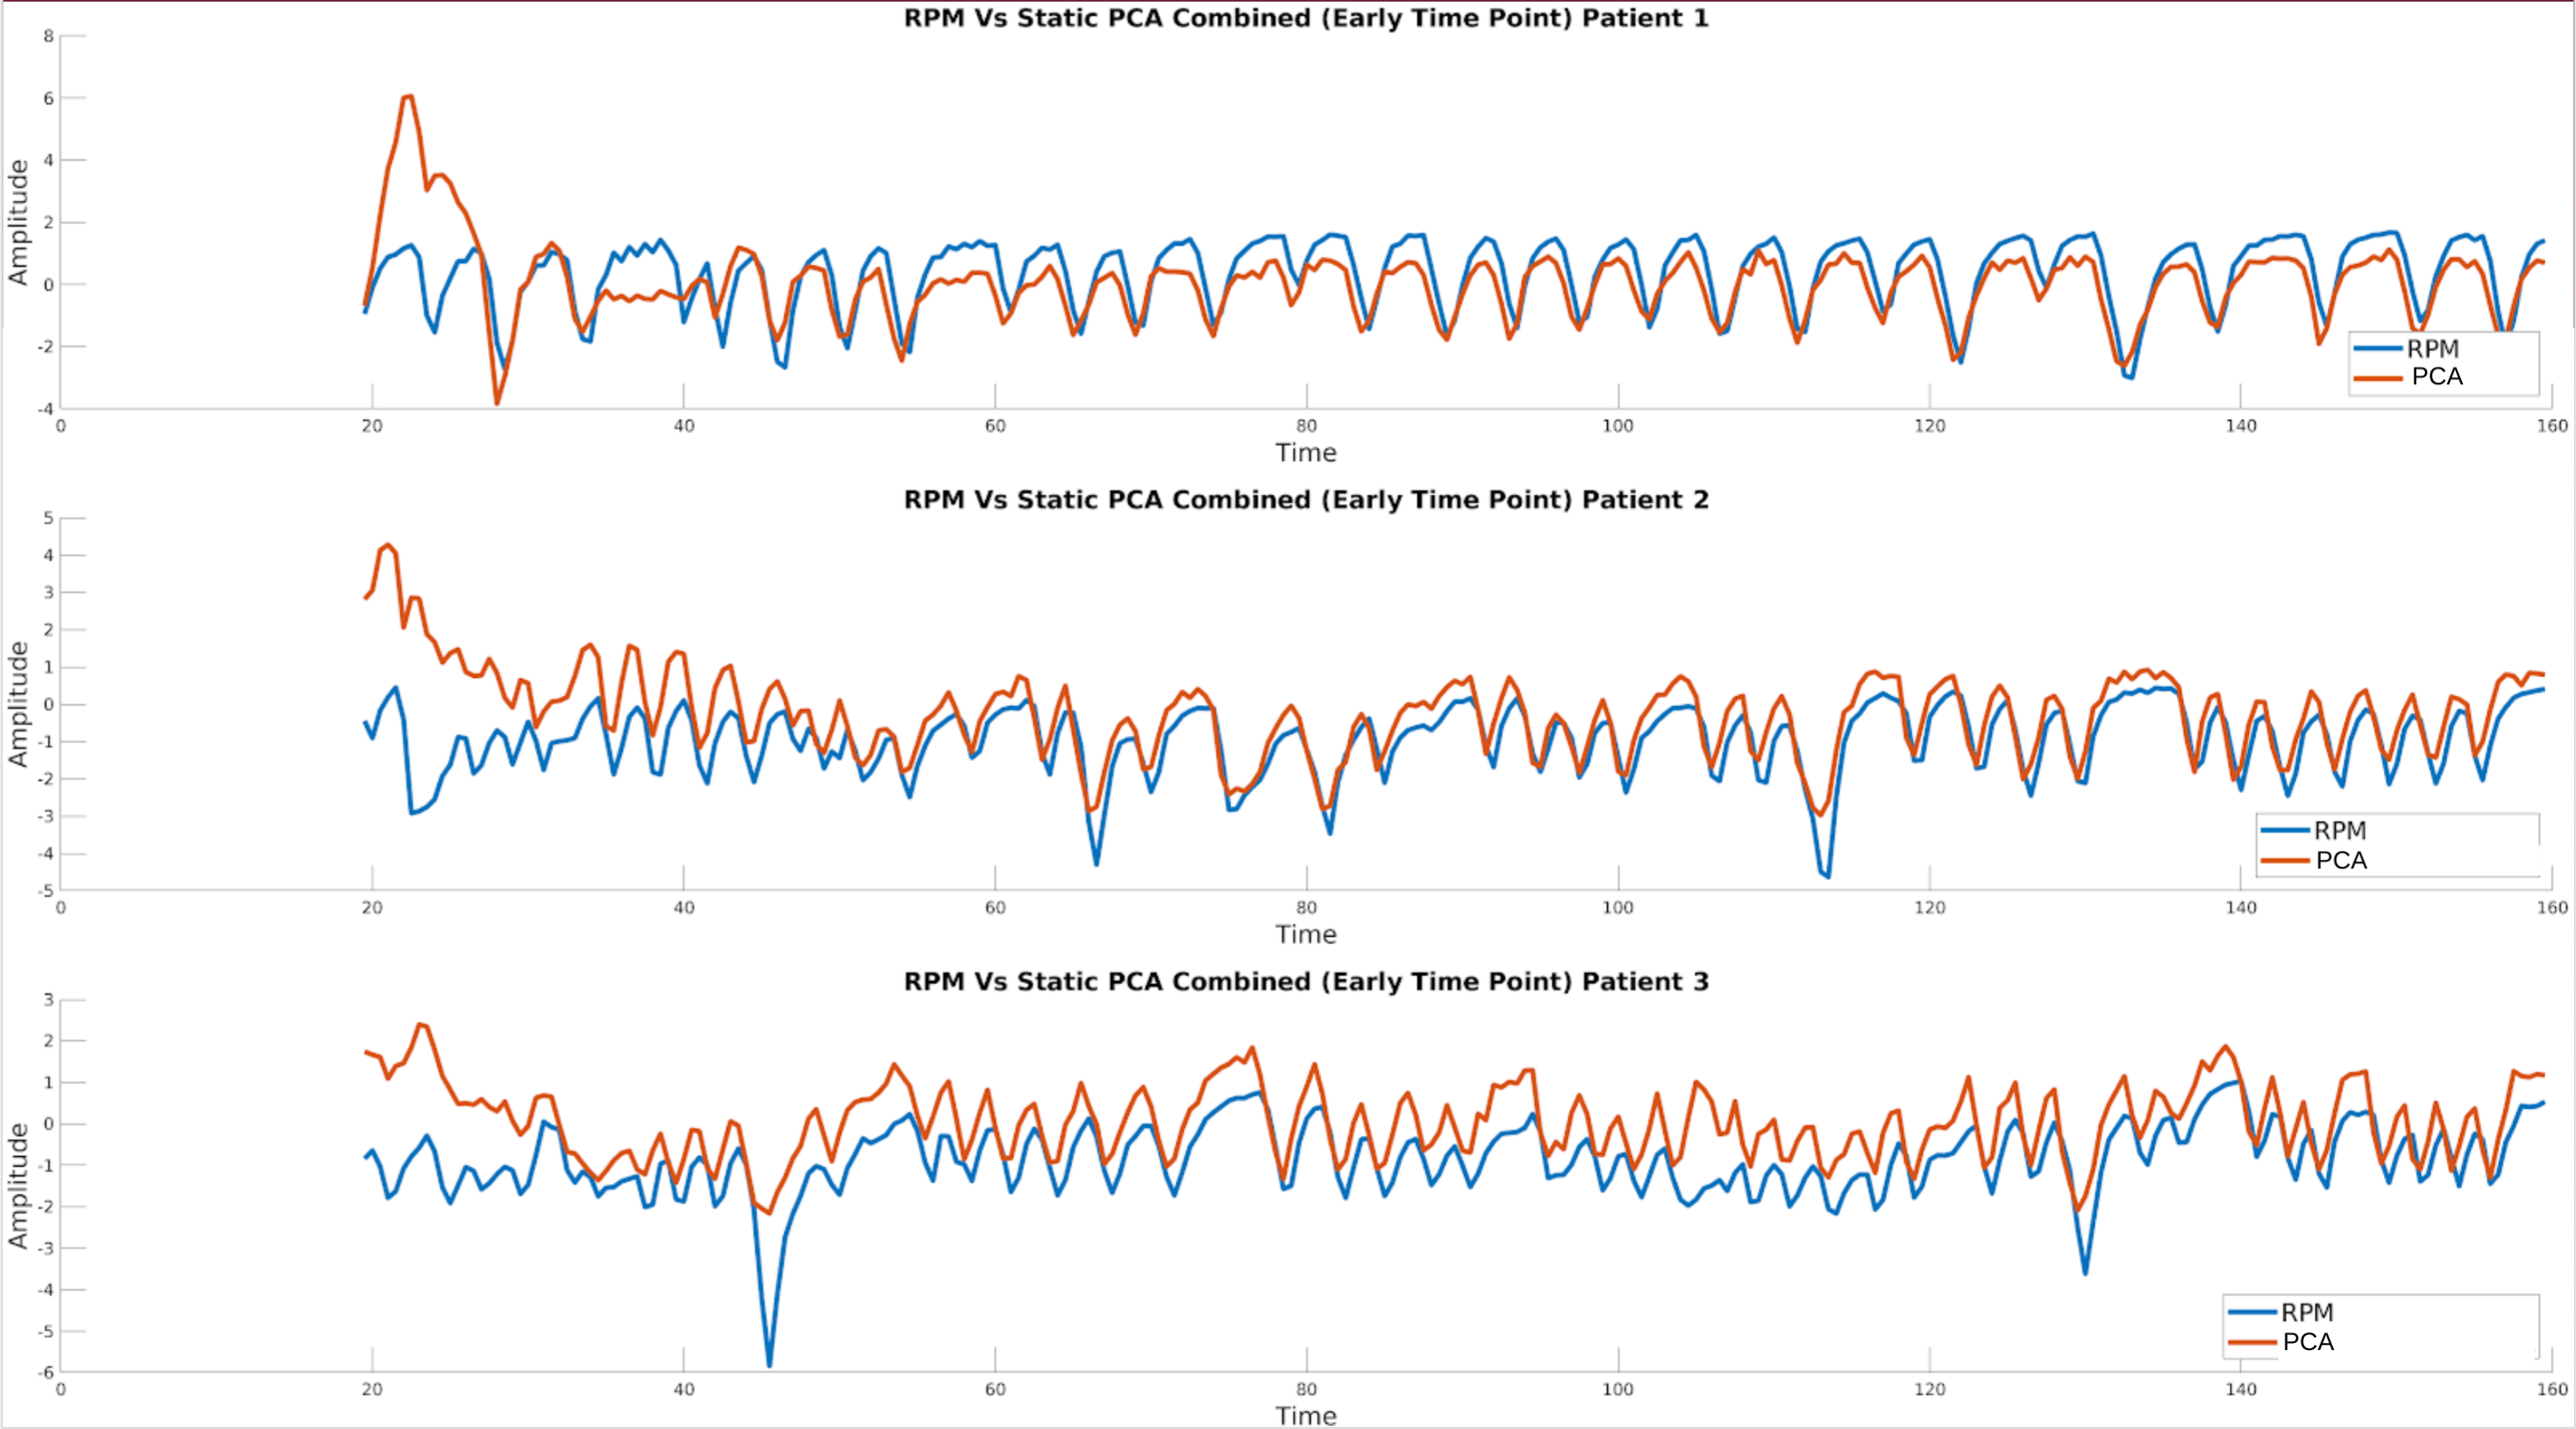
\includegraphics[width=1.0\linewidth]{figures/data_driven_surrogate_signal_extraction_results_1_combined_surrogate_signal.png}
        
        \captionsetup{singlelinecheck=false}
        \caption{
            A visual comparison between the \gls{RPM} \gls{SS} and the \gls{SS} from the static \gls{PCA} method by combining the first $20$ \glspl{PC} for three patients between \SI{20}{\second} and \SI{160}{\second}. The three patients shown here are the ones on which parameters for the method were optimised. Here no pre- or post-processing is used.
        }
        \label{fig:pca_data_driven_surrogate_signal_extraction_methods_for_dynamic_pet_results_with_and_without_pre_and_post_processing_appendix_combined_surrogate_signal}
    \end{figure}
    
    \begin{figure}
        \centering
        
        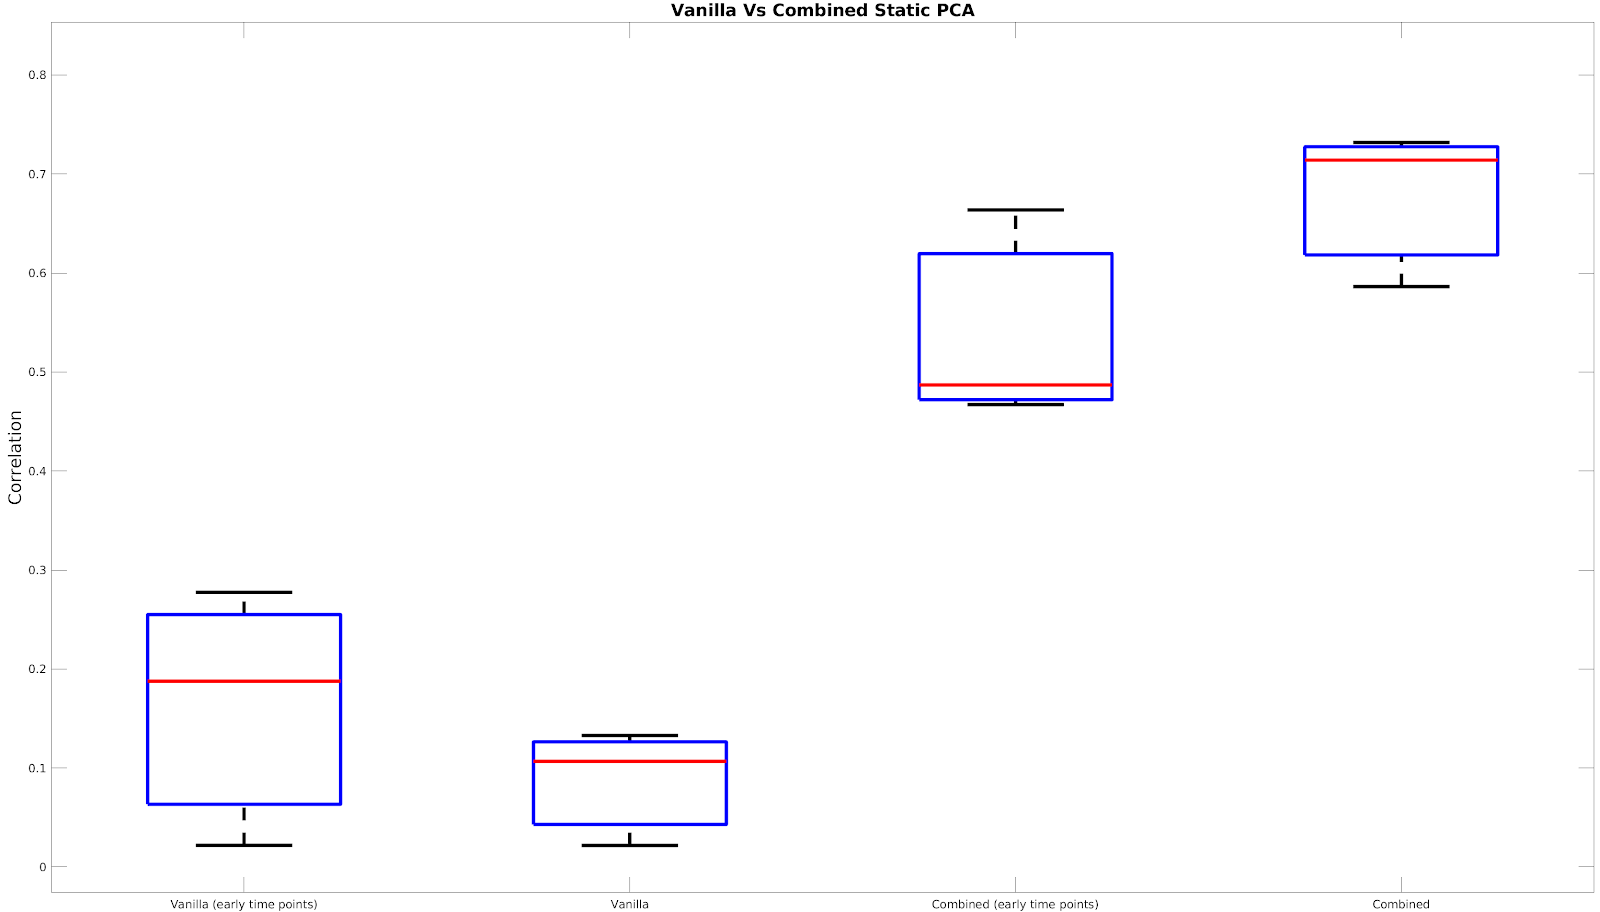
\includegraphics[width=1.0\linewidth]{figures/data_driven_surrogate_signal_extraction_results_1_box_plot.png}
        
        \captionsetup{singlelinecheck=false}
        \caption{
            A box plot of the \gls{CC} between static \gls{PCA} method both when using only the first \gls{PC} and by combining the first $20$ \glspl{PC} for all patients between \SI{20}{\second} and \SI{160}{\second} and for the entire acquisition. The parameters used here were optimised for and frozen based on the results shown in other diagrams on three patients. Here no pre- or post-processing is used.
        }
        \label{fig:pca_data_driven_surrogate_signal_extraction_methods_for_dynamic_pet_results_with_and_without_pre_and_post_processing_appendix_box_plot}
    \end{figure}
    
    \begin{figure}
        \centering
        
        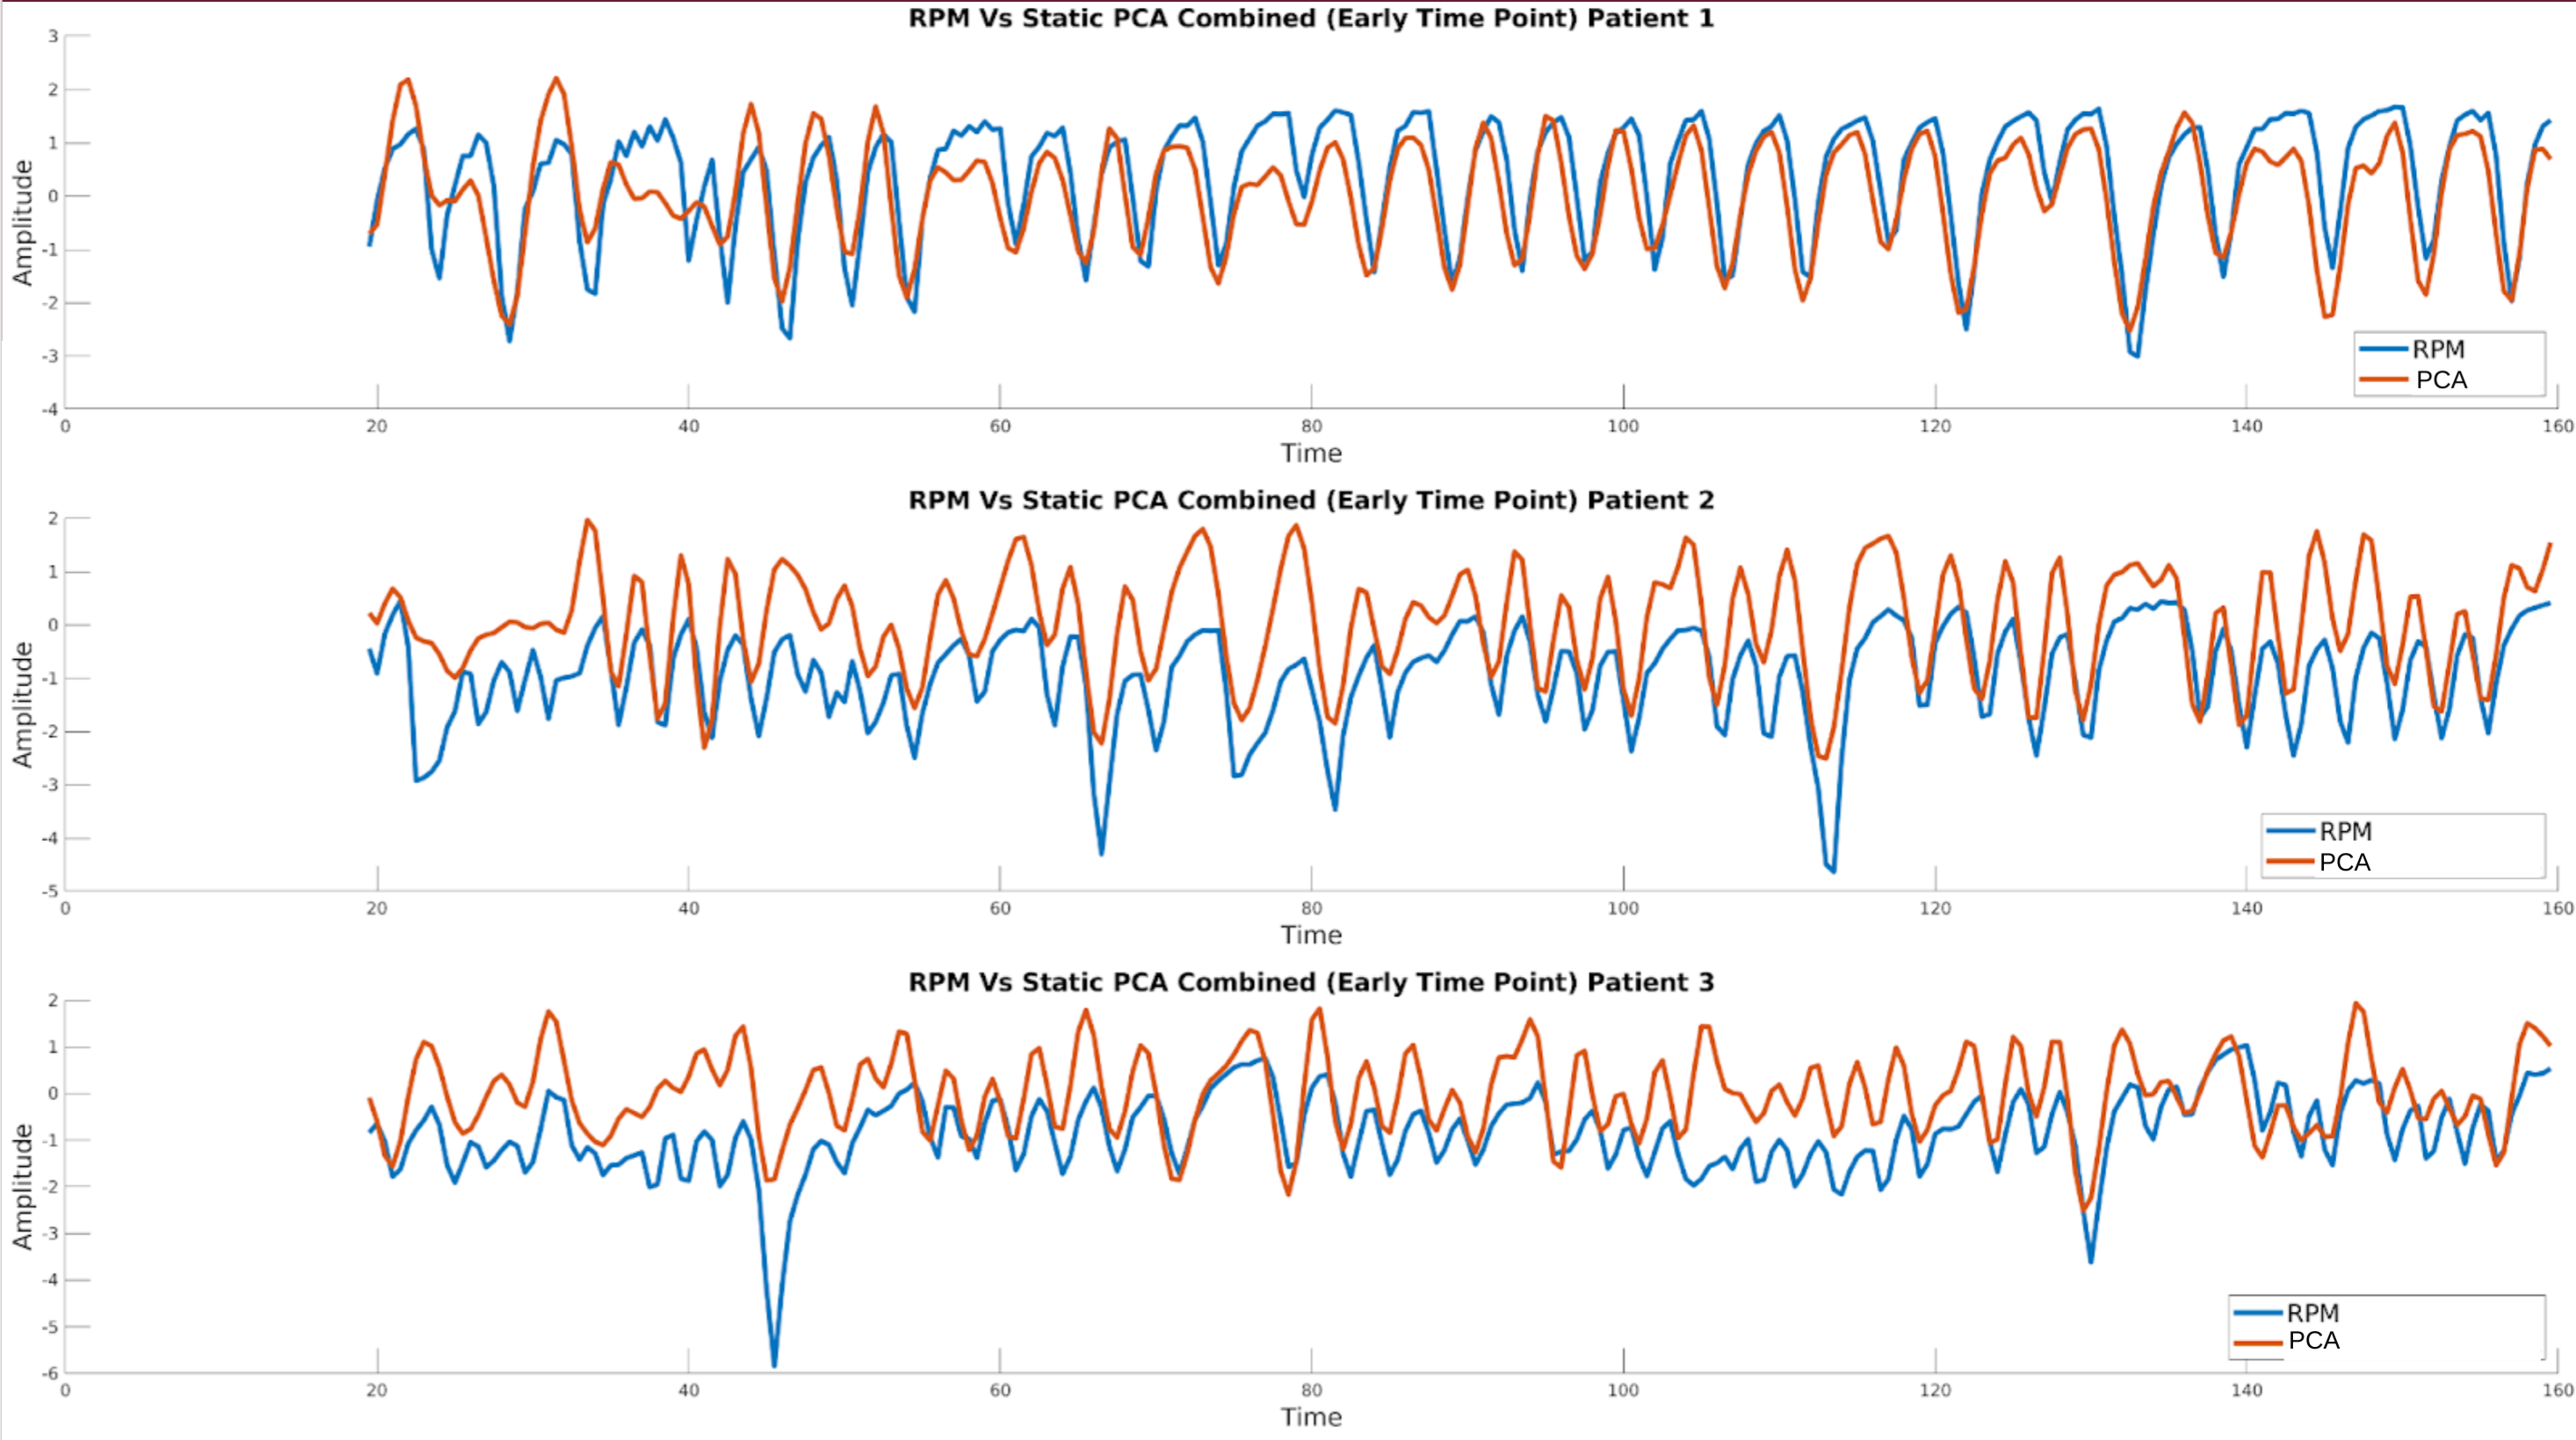
\includegraphics[width=1.0\linewidth]{figures/data_driven_surrogate_signal_extraction_results_1_combined_surrogate_signal_processed.png}
        
        \captionsetup{singlelinecheck=false}
        \caption{
            A visual comparison between the \gls{RPM} \gls{SS} and the \gls{SS} from the static \gls{PCA} method by combining the first $20$ \glspl{PC} for three patients between \SI{20}{\second} and \SI{160}{\second}. The three patients shown here are the ones on which parameters for the method were optimised. Here pre- and post-processing are used.
        }
        \label{fig:pca_data_driven_surrogate_signal_extraction_methods_for_dynamic_pet_results_with_and_without_pre_and_post_processing_appendix_combined_surrogate_signal_processed}
    \end{figure}
    
    \begin{figure}
        \centering
        
        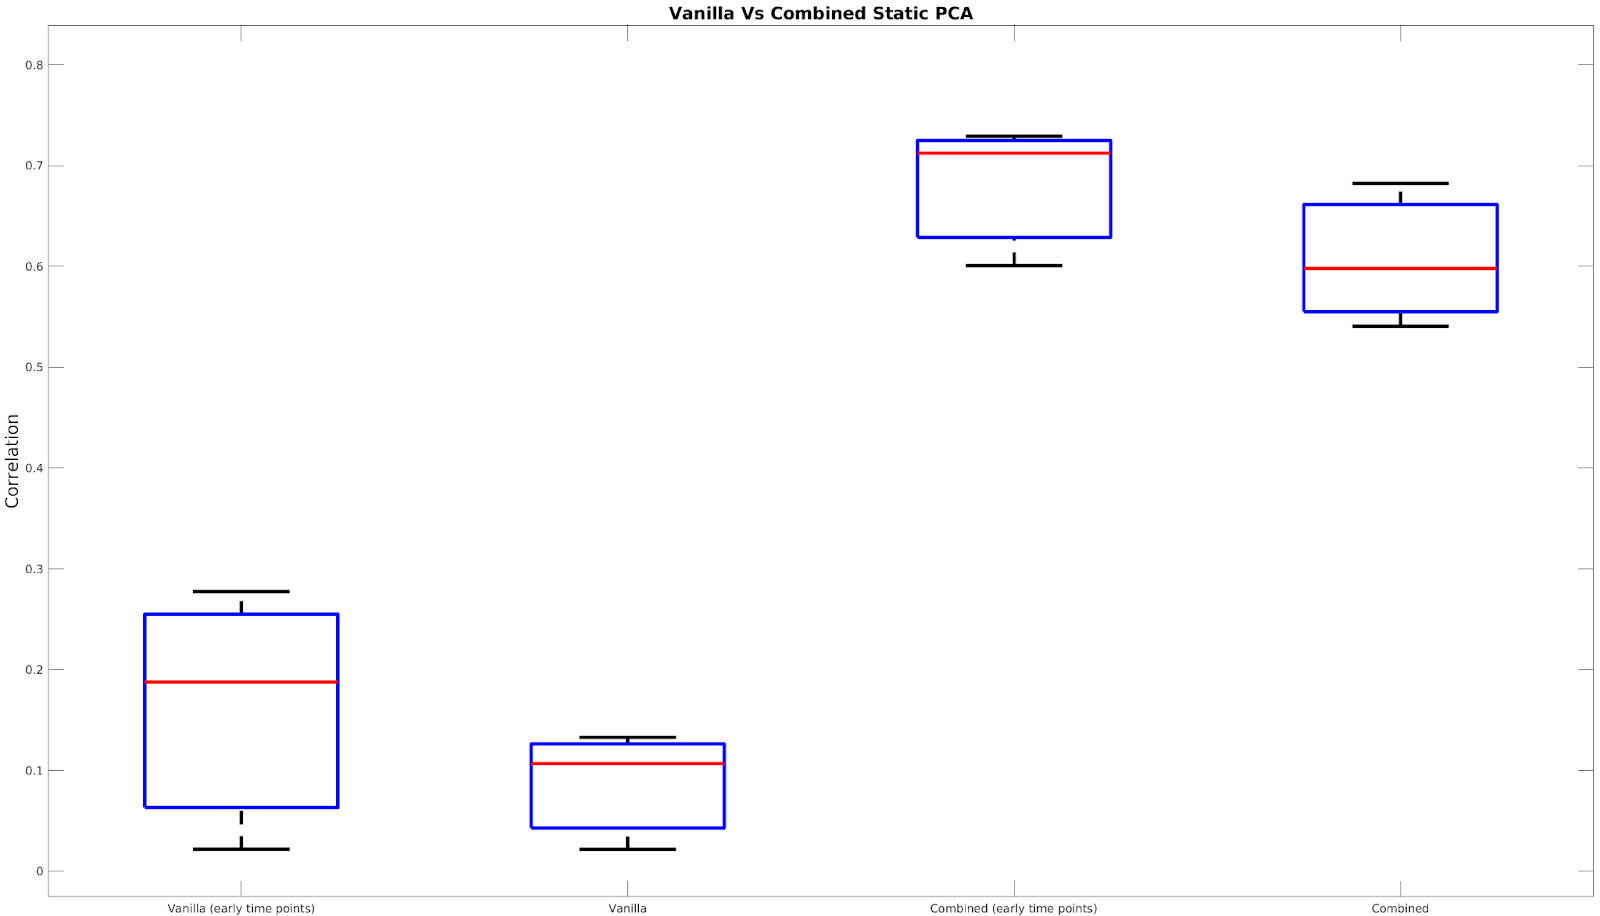
\includegraphics[width=1.0\linewidth]{figures/data_driven_surrogate_signal_extraction_results_1_box_plot_processed.png}
        
        \captionsetup{singlelinecheck=false}
        \caption{
            A box plot of the \gls{CC} between static \gls{PCA} method both when using only the first \gls{PC} and by combining the first $20$ \glspl{PC} for all patients between \SI{20}{\second} and \SI{160}{\second} and for the entire acquisition. The parameters used here were optimised for and frozen based on the results shown in other diagrams on three patients. Here pre- and post-processing are used.
        }
        \label{fig:pca_data_driven_surrogate_signal_extraction_methods_for_dynamic_pet_results_with_and_without_pre_and_post_processing_appendix_box_plot_processed}
    \end{figure}
    
    Results presented here are only for the static \gls{PCA} case. For results presented here parameters were selected on a subset of the data (specifically three randomly selected scans) before being applied across the entire data set. A plot of the \gls{SS} for static \gls{PCA} using only one \gls{PC} for three patients at early time points can be seen in~\Fref{fig:pca_data_driven_surrogate_signal_extraction_methods_for_dynamic_pet_results_with_and_without_pre_and_post_processing_appendix_vanilla_surrogate_signal}. It can be observed in this example that only using the static \gls{PCA} method and one \gls{PC} does not give satisfactory results at early time points. A plot of the \gls{SS} for static \gls{PCA} using a combination of the first $20$ \glspl{PC} for three patients at early time points can be seen in~\Fref{fig:pca_data_driven_surrogate_signal_extraction_methods_for_dynamic_pet_results_with_and_without_pre_and_post_processing_appendix_combined_surrogate_signal}, here no pre- or post-processing is used. Here for all patients from very early in the acquisition it can be seen that the method gives comparable results to the \gls{RPM}. A plot of the \gls{SS} for static \gls{PCA} using a combination of the first $20$ \glspl{PC} for three patients at early time points can be seen in~\Fref{fig:pca_data_driven_surrogate_signal_extraction_methods_for_dynamic_pet_results_with_and_without_pre_and_post_processing_appendix_combined_surrogate_signal_processed}, here pre- and post-processing are used. The parameters for the processing were optimised solely to improve the \gls{CC} for early time points, as such it can be seen that some inter-window variation has been removed (from parallel compression).
    
    A box plot of the \gls{CC} of the \gls{SS} for static \gls{PCA} using only one \gls{PC} compared to the \gls{RPM} and the \gls{CC} of the \gls{SS} for static \gls{PCA} using a combination of the first $20$ \glspl{PC} compared to the \gls{RPM} for all patients at both early time points and all time points and  can be seen in~\Fref{fig:pca_data_driven_surrogate_signal_extraction_methods_for_dynamic_pet_results_with_and_without_pre_and_post_processing_appendix_box_plot}, here no pre- or post-processing is used. Here the improvement by incorporating multiple \glspl{PC} is most apparent. A box plot of the \gls{CC} of the \gls{SS} for static \gls{PCA} using only one \gls{PC} compared to the \gls{RPM} and the \gls{CC} of the \gls{SS} for static \gls{PCA} using a combination of the first $20$ \glspl{PC} compared to the \gls{RPM} for all patients at both early time points and all time points and  can be seen in~\Fref{fig:pca_data_driven_surrogate_signal_extraction_methods_for_dynamic_pet_results_with_and_without_pre_and_post_processing_appendix_box_plot_processed}, here pre- and post-processing are used. The parameters for the processing were optimised solely to improve the \gls{CC} for early time points, as such it can be seen that the \gls{CC} drops from no processing to processing for the entire acquisition, it can be assumed this effect is similar to minimising variance at the expense of bias or vice versa.
